\documentclass[twoside]{article}
\usepackage{mdframed}
\usepackage[hmarginratio=1:1,top=32mm,columnsep=20pt]{geometry} % Document margins
\usepackage{multicol} % Used for the two-column layout of the document
\usepackage[hang, small,labelfont=bf,up,textfont=it,up]{caption} % Custom captions under/above floats in tables or figures
\usepackage{booktabs} % Horizontal rules in tables
\usepackage{float} % Required for tables and figures in the multi-column environment - they need to be placed in specific locations with the [H] (e.g. \begin{table}[H])
\usepackage{hyperref} % For hyperlinks in the PDF
\usepackage{amsmath,amsthm,amssymb}
\usepackage{lettrine} % The lettrine is the first enlarged letter at the beginning of the text
\usepackage{paralist} % Used for the compactitem environment which makes bullet points with less space between them
\usepackage{tikz}
\usepackage{esint}
\usepackage{centernot}
\usepackage{lmodern}
\usetikzlibrary{3d}
\usetikzlibrary{patterns,calc,hobby}
\usetikzlibrary{decorations.pathreplacing}
\tikzset{
	partial ellipse/.style args={#1:#2:#3}{
		insert path={+ (#1:#3) arc (#1:#2:#3)}
	}
}
\usepackage{xcolor}

\usepackage{fancyhdr} % Headers and footers
\pagestyle{fancy} % All pages have headers and footers
\fancyhead{} % Blank out the default header
\fancyfoot{} % Blank out the default footer
\fancyhead[C]{Jimmy Yue $\bullet$ Statistics $\bullet$ Jimmy Yue} % Custom header text
\fancyfoot[RO,LE]{\thepage} % Custom footer text

\newmdenv[skipabove=7pt,
rightline=false,
leftline=true,
topline=false,
bottomline=false,
skipbelow=5pt,
linecolor=black,
innerleftmargin=5pt,
innerrightmargin=5pt,
innertopmargin=5pt,
leftmargin=0cm,
rightmargin=0cm,
linewidth=4pt,
innerbottommargin=5pt]{cBox}

\theoremstyle{definition}
\newtheorem*{solutionT}{Solution}

\newenvironment{solution}{\begin{cBox}\begin{solutionT}}{\hfill{\scriptsize\ensuremath{\square}}\end{solutionT}\end{cBox}}

%%%%%%%%%%%%%%%%%%%%%%%%%%%%%%%%%%%%%%%%%%%%%%%%%%%%%%%%%%%%%%%%%%%%%%%%%%%%%%%%%%%%%%%%%%%%
\newcommand{\vect}[1]{\vec{\pmb{#1}}}
\newcommand{\uvect}[1]{\hat{\mathbf{#1}}}
\newcommand{\leviciv}{\epsilon_{ijk}}

\newmdenv[skipabove=7pt,
rightline=false,
leftline=true,
topline=false,
bottomline=false,
skipbelow=5pt,
linecolor=black,
innerleftmargin=5pt,
innerrightmargin=5pt,
innertopmargin=5pt,
leftmargin=0cm,
rightmargin=0cm,
linewidth=4pt,
innerbottommargin=7,
backgroundcolor=light-gray]{dBox}



\theoremstyle{definition}
\newtheorem*{proof1}{Definition}

\newenvironment{ddef}{\begin{dBox}\begin{proof1}}{\hfill{\scriptsize}\end{proof1}\end{dBox}}
\newcommand{\pdif}[2]{\frac{\partial#1}{\partial#2}}
\definecolor{light-gray}{gray}{0.85}
%----------------------------------------------------------------------------------------
%-	TITLE SECTION
%----------------------------------------------------------------------------------------

\title{\vspace{-15mm}\fontsize{24pt}{10pt}\selectfont\textbf{Statistics - Week 5}} % Article title

\author{
\large
\textsc{Jimmy Tsz Ming Yue}\thanks{440159151}\\[2mm] % Your name
\normalsize University of Sydney \\ % Your institution
\normalsize \href{mailto:jyue6728@uni.sydney.edu.au}{jyue6728@uni.sydney.edu.au} % Your email address
\vspace{-5mm}
}
\date{}

%----------------------------------------------------------------------------------------

\usepackage{Sweave}
\begin{document}
\Sconcordance{concordance:week5.tex:week5.Rnw:%
1 359 1 1 3 2 0 4 1 1 2 1 0 4 1 1 2 4 0 1 2 7 1 1 2 12 0 1 1 5 0 4 1 11 %
0 1 1 5 0 2 1 6 0 1 2 7 1 1 2 1 0 1 1 1 5 7 0 2 2 19 0 1 11 13 0 1 4 4 %
0 1 7 5 0 1 1 18 0 1 1 21 0 1 11 9 0 1 1 3 0 1 7 5 0 1 2 22 0 1 9 8 0 1 %
1 3 0 1 3 1 0 1 2 1 0 1 2 1 0 1 2 1 0 1 1 4 0 1 2 4 1 1 2 1 0 2 1 5 0 1 %
1 5 0 1 1 4 0 1 2 9 1}


\maketitle % Insert title

\thispagestyle{fancy} % All pages have headers and footers
\hrule \smallskip

\noindent Semester 2 \quad Statistics \hspace{10.5
cm} 2018
\smallskip
\hrule
\smallskip
\tableofcontents

\section{Basic Principles of Classification}

For each object associated with a class label (or response ) $y \in \left\{ 1,2, \dots, K  \right\}$ and a feature vector (vector of predictor variables) of $N$ measurements: $X = \left( x_1, \dots, x_N \right)$ the aim is to classify $y$ using $X$. 

\subsection{Classification vs Clustering}

There is a difference between classification and clustering;

\begin{enumerate}
	\item Clustering: classes are unknown and is the object of discovery from the data. It is a form of  unsupervised learning
	\item Classification: classes are predefined, and the aim is tu se a training or learning set of labelled objects to form a classifier for classification of future observations. It is a form of supervised learning
\end{enumerate}


\subsection{Classification vs Regression}

\begin{enumerate}
	\item Regression: No class definition, the response variable is a continuous value. The relationship between explanatory variables and the response variable is the subject of the model.
	\item Classification: Samples are predefined to be from a given class. Classification models produce a continous valued prediction, which is usually in the form of a probability, or probability distribution. A predicted class is required in order to make a decision. 
\end{enumerate}

\subsection{Classification}

INSERT PICTURE HERE:

Classification rule determined by following factors:
\begin{enumerate}
	\item Classification procedure,
	\item Feature selection,
	\item Parameters (both pre-determined and estimable)
	\item Distance measures
	\item Aggregation methods
\end{enumerate}
One can think of the classification rule as a black box, some methods may provide more insight into the box. Performance assessments needs to be looked at for all classification rules. 

\section{Two class classification}

Examples of the two class problems include:

\begin{enumerate}
	\item Email: Spam/Not Spam
	\item Tumour: Malignant/Benigh 
\end{enumerate}

The general idea behind the two class problems is to label a sample as $y \in \left\{ 0,1 \right\}$, where \begin{enumerate}
	\item $0$: `` negative class''
	\item $1$: ``positive class''
\end{enumerate}

Generate a threshold classifier output $h_\theta(x)$ at 0.5, then:
\begin{enumerate}
	\item if $h_\theta(x) > 0.5$, predict $y=1$
	\item if $h_\theta(x) < 0.5$, predict $y=0$.
\end{enumerate}

This generates the question as to why we do not simply use simple linear regression. This can be easily seen through the example: When $y$ only takes on valuesof $0$ and $1$, standard linear regression will produce values greater than $1$ and values of $y$ between $0$ and $1$. There are other problems:

\begin{enumerate}
	\item The regression line $\beta_0 + \beta_1 x$ can take on any value between negative and positive infinity. For example in the diagnosis problem, $y$ can only take on two possible values $0$ and $1$. Therefore a simple regression line almost always predicts the wrong value for $y$ in classification problems. 


\end{enumerate}
As such we need another type of regression; of which the Logistic Regression can be motivated;
\section{Logistic Regression}

\begin{ddef}
	The logistic regression model is defined as:

	\begin{equation}
		\log\left( \frac{p}{1-p} \right) = \beta_0 + \beta_1x_1 + \dots + \beta_px_p = \theta^T\vec{x}
	\end{equation} 

	For which solving for $p$ we get;

	\begin{align}
		p & = \text{Pr}(y=1|\vec{x})\\
		& = h_\theta(\vec{x})\\
		& = g(\theta^T(\vec{x}))\\
			& = \frac{1}{1+ e^{-\theta^T \vec{x}}}
	\end{align}
\end{ddef}

\subsection{Logistic Regression: Decision boundary}

We can construct the notion of a decision boundary from the  above equations; 

We predict $y=1$ if $\theta^T x \geq 0$. NEEDS CLARIFICATION ON THIS POINT


\subsection{Maximum likelihood estimation of theta  with single predictor} 

From above we have that;

\begin{align}
	\text{Pr} (y=1|x) & = g(\theta_0 + \theta_1x)
	\intertext{Then from the axioms of probability the complementary event:}
	\text{Pr} (y=0|x) & = 1 - g(\theta_0 + \theta_1x)\\
	\text{Pr} (y|x) & = \left[ g(\theta_0 + \theta_1x) \right]^y\left[ 1-g(\theta_0 + \theta_1x) \right]^{1-y}
	\intertext{Then the likelihood function of $n$ samples``}
	L & = \prod^n_{i=1} \left[ g(\theta_0 + \theta_1 x_i \right]^{y_i}\left[ 1 - g(\theta_0 + \theta_1 x_1) \right]^{1-y_i}
	\intertext{If we then take the log of both sides to find the log-likelihood:}
	\text{log}(L) & = \sum^n_{i=1} y_i \text{log} \left[ g(\theta_0 + \theta_1 x_i \right] + (1-y_i)\text{log}\left[ 1 - g(\theta_0 + \theta_1 x_1) \right]
		\intertext{Then the partial derivatives:}
		\pdif{\text{log}(L)}{\theta_0} & = 0\\
\pdif{\text{log}(L)}{\theta_1} & = 0
\end{align}

\section{Linear Discriminant Analysis} 

Linear Discriminant Analysis or LDA, undertakes the same task as Logistic Regression. It classifies data based on categorical variables. For example;

\begin{enumerate}
	\item Malignant or benign cancer;
	\item Making profit in a business or not
	\item Buying a product or not
	\item Satisfised customer or not
\end{enumerate}

\subsection{Logistic Regression vs LDA formulation}

Logistic Regressions model the probability of $Y$ being from the $k$-th class as:

\begin{equation}
	p(X) = \text{Pr}(Y = k|X=x) = \frac{e^{\beta_0 + \beta_1X}}{ 1 + e^{\beta_0 + \beta_1X}}
\end{equation}

However through Bayes' Theorem, we have that:

\begin{equation}
	p(X) = \text{Pr} (Y = k|X=x)  = \frac{\pi_k f_k(x)}{\sum^K_{i=1} \pi f_l(x)}
\end{equation}

where:

\begin{enumerate}
	\item $\pi_k$: Probability of coming from class $k$ which is also called the prior 
	\item $f_k(x)$: Density function for $X$ given that $X$ is an observation from class $k$.
\end{enumerate}

\subsection{LDA estimations}

LDA estimates $\pi_k$ and $f_k(x)$. We can estimate these parameters to compute $p(X)$. The most common model for $f_k(x)$ is the normal density (LDA):

\begin{equation}
	f_k(x) = \frac{1}{\sqrt{2\pi} \sigma_k}e^{-\frac{1}{2\sigma^2_k}(x-\mu_k)^2} 
\end{equation}

Using this density, we only need to estimate three quantities to compute $p(X)$: 

\begin{enumerate}
	\item $\mu_k$
	\item $\sigma^2_k$
	\item $\pi_k$
\end{enumerate}

\subsection{Using training data set for estimation}

The mean $\mu_k$ can be estimated through the averaging of all training observations from the $k$-th class. The variance $\sigma_k^2$ can be estimated as the weighted average of variances of all $k$ classes. And lastly we have that $\pi_k$ can be estimated as the proportion of the training observations that belong to the $k$-th class. 

\begin{align}
	\hat{\mu_k} & = \frac{1}{n_k} \sum_{i:y_i =k} x_i\\
	\hat{\sigma^2} & = \frac{1}{n-K} \sum^K_{k=1} \sum_{i:y_i = k} (x_i - \hat{\mu_k})^2\\
	\hat{\pi_k} & = \frac{n_k}{n}
\end{align}

Let us present a simple example:
\begin{cBox}
	Suppose we have only one predictor, then let two normal density functions denoted $f_1(x)$ and $f_2(x)$ represent two distinct classes. These two density functions overlap, so there is some uncertainty about the class to which an observation with an unknown class belongs. The dashed vertical line represents Bayes' decision boundary;

	INSERT PICTURE HERE
\end{cBox}

\subsection{Deriving LDA for one predictor}

Assuming that we are working with only one predictor:

\begin{align}
	f_k(x) & = \frac{1}{\sqrt{2\pi\sigma_k}}e^{-\frac{1}{2\sigma^2_k}(x-\mu_k)^2}\\
p_k(x) = \text{Pr}(y=k|x) & = \frac{\pi_k \frac{1}{\sqrt{2\pi\sigma_k}}e^{-\frac{1}{2\sigma^2_k}(x-\mu_k)^2}}{\sum^K_{l=1}\pi_l\frac{1}{\sqrt{2\pi\sigma_k}}e^{-\frac{1}{2\sigma^2_k}(x-\mu_k)^2}}
\intertext{Taking the log}
\text{log}(p_k(x)) & = x \frac{\mu_k}{\sigma^2} - \frac{\mu^2_k}{2\sigma^2} + \text{log}(\pi_k)
\end{align}

\subsection{LDA decision boundary}

If $K=2$ and $\pi_1 = \pi_2$, then assigns an observation to class $1$ if:

\begin{align}
	\text{log}(p_1(x)) & > \text{log}(p_2(x))\\
x \frac{\mu_1}{\sigma^2} - \frac{\mu^2_1}{2\sigma^2} + \text{log}(\pi_1)  - x \frac{\mu_2}{\sigma^2} - \frac{\mu^2_2}{2\sigma^2} + \text{log}(\pi_2) & > 0\\ 
2x(\mu_1 - \mu_2) & > \mu^2_1 - \mu^2_2
\end{align}

\begin{ddef}
	Therefore we have the decision boundary for the LDA to be defined as:
	\begin{align}
		x & = \frac{\mu_1^2 -\mu^2_2}{2(\mu_1 - \mu_2)}\\		& = \frac{\mu_1 + \mu_2}{2}	
	\end{align}

	T
\end{ddef}

\subsection{LDA for more than one learning feature}

\begin{ddef}
	Now that we have defined LDA for more than one feature, let us attempt to extend this to multiple learning features;
Let us first present again the one feature LDA:
\begin{align}
	\text{log}(p_k(x)) & = x \frac{\mu_k}{\sigma^2} - \frac{\mu^2_k}{2\sigma^2} + \text{log}(\pi_k)
	\intertext{Then we have for more than one feature:}
	\text{log}(p_k(\vec{x})) & = \vec{x}^T \vec{\Sigma}^{-1} \frac{\mu_k}{\sigma^2} - \frac{1}{2}\vec{\mu_k}\vec{\Sigma}^{-1}\vec{mu_k} + \text{log}(\pi_k)
\end{align}
\end{ddef}

\subsection{Why not use logistic regression}

Logistic regression is unstable when the classes are well separated. In the case where $n$ is small, and the distribution of predictors $X$ is approximately normal, then LDA is more stable than Logistic Regression.  Usually LDA is more popular when we have more than two response classes.

\subsection{LDA vs Logistic Regression}

Similarity: Both Logistic Regression and LDA produce linear boundaries. 

Difference: LDA assumes that the observations are drawn from the normal distribution with common variance in each class, while logistic regression does not have this assumption. 

LDA would do better than Logistic Regression if the assumption of normality holds, otherwise logistic regresion may outperform LDA

\section{Classification evaluation based on class labels Training and testing errors} 

\begin{ddef}
	\textbf{Training error rate} 
	\begin{equation}
		\frac{1}{N} \sum^N_{i=1} I(y_i \neq \hat{y_i})
	\end{equation}
\end{ddef}a

\begin{ddef}
	\textbf{Test error rate}
	\begin{equation}
		\frac{1}{T} \sum^T_{t=1} I(y_t \neq \hat{y_i})
		\label{<+label+>}
	\end{equation}<++>
\end{ddef}

Often the best classifier is the one for which the test error is the smallest. It should be noted that test error not be used for classifcation evaluation

\section{Tutorial}
\begin{Schunk}
\begin{Sinput}
> # create positive class sample with 2 descriptive features
> set.seed(3)
> f1 <- rnorm(100, mean=6, sd = 1.2)
> set.seed(4)
> f2 <- rnorm(100, mean=6, sd = 1.2)
> P.data <- cbind(f1, f2)
> # create positive class sample with 2 descriptive features
> set.seed(7)
> f1 <- rnorm(300, mean=4, sd = 1.2)
> set.seed(8)
> f2 <- rnorm(300, mean=4, sd = 1.2)
> N.data <- cbind(f1, f2)
> # combine all samples
> data.mat <- data.frame(rbind(P.data, N.data), Class=rep(c(1, 0), time=c(nrow(P.data), nrow(N.data))))
\end{Sinput}
\end{Schunk}

The above code will create a dataset with two class and two features, each follows a normal distribution.

\begin{enumerate}
  \item Partition the data into $80\%$ for model training (training set) and $20\%$ for model testing (test set).
  
  \begin{solution}
  First load the caret package to deal with paritioning data sets:
\begin{Schunk}
\begin{Sinput}
> head(data.mat)
\end{Sinput}
\begin{Soutput}
        f1       f2 Class
1 4.845680 6.260106     1
2 5.648969 5.349009     1
3 6.310546 7.069374     1
4 4.617442 6.715177     1
5 6.234939 7.962742     1
6 6.036149 6.827131     1
\end{Soutput}
\begin{Sinput}
> dim(data.mat)
\end{Sinput}
\begin{Soutput}
[1] 400   3
\end{Soutput}
\begin{Sinput}
> library(caret)
> inTrain <- createDataPartition(data.mat$Class, p = .8)[[1]]
> data.train <- data.mat[inTrain, ]
> head(data.train)
\end{Sinput}
\begin{Soutput}
        f1       f2 Class
1 4.845680 6.260106     1
2 5.648969 5.349009     1
3 6.310546 7.069374     1
5 6.234939 7.962742     1
6 6.036149 6.827131     1
8 7.339932 5.744227     1
\end{Soutput}
\begin{Sinput}
> dim(data.train)
\end{Sinput}
\begin{Soutput}
[1] 320   3
\end{Soutput}
\begin{Sinput}
> data.test <- data.mat[-inTrain, ]
> dim(data.test)
\end{Sinput}
\begin{Soutput}
[1] 80  3
\end{Soutput}
\end{Schunk}
      
  \end{solution}
  \item Train a Logistic Regression, a LDA and a kNN (try different $k$ value) classifier using
training dataset. Compare their performance using test dataset. 
    
   \begin{solution} 
   Let us first do the Logistic Regression using glm;
   
\begin{Schunk}
\begin{Sinput}
> set.seed(1)
> data.train$Class <- as.factor(data.train$Class)
> logisticRegFull <- train(Class ~ f1,
+                      data = data.train,
+                      method = "glm",
+                      trControl = trainControl(method = "repeatedcv", 
+                                               repeats = 5))
\end{Sinput}
\end{Schunk}

\begin{Schunk}
\begin{Sinput}
> logisticRegFull
\end{Sinput}
\begin{Soutput}
Generalized Linear Model 

320 samples
  1 predictor
  2 classes: '0', '1' 

No pre-processing
Resampling: Cross-Validated (10 fold, repeated 5 times) 
Summary of sample sizes: 288, 288, 288, 288, 288, 288, ... 
Resampling results:

  Accuracy  Kappa    
  0.834375  0.5139071
\end{Soutput}
\end{Schunk}
\begin{Schunk}
\begin{Sinput}
> PredictFunc <- function(logisticReg) {
+   Results <- data.frame(obs = data.test$Class)
+   Results$prob <- predict(logisticReg, data.test, type = "prob")[, "1"]
+   Results$pred <- predict(logisticReg, data.test)
+   Results$Label <- ifelse(Results$obs == "1", 
+                               "True Outcome: 1", 
+                               "True Outcome: 0")
+   return(Results)
+ }
> 
\end{Sinput}
\end{Schunk}
\begin{Schunk}
\begin{Sinput}
> ResultsFull <- PredictFunc(logisticRegFull)
\end{Sinput}
\end{Schunk}
\begin{Schunk}
\begin{Sinput}
> LDAFull <- train(Class ~ .,
+                      data =data.train,
+                      method = "lda",
+                      trControl = trainControl(method = "repeatedcv", 
+                                               repeats = 5))
> summary(LDAFull)
\end{Sinput}
\begin{Soutput}
            Length Class      Mode     
prior       2      -none-     numeric  
counts      2      -none-     numeric  
means       4      -none-     numeric  
scaling     2      -none-     numeric  
lev         2      -none-     character
svd         1      -none-     numeric  
N           1      -none-     numeric  
call        3      -none-     call     
xNames      2      -none-     character
problemType 1      -none-     character
tuneValue   1      data.frame list     
obsLevels   2      -none-     character
param       0      -none-     list     
\end{Soutput}
\begin{Sinput}
> LDAFull$finalModel
\end{Sinput}
\begin{Soutput}
Call:
lda(x, grouping = y)

Prior probabilities of groups:
   0    1 
0.75 0.25 

Group means:
        f1       f2
0 4.130876 3.904459
1 6.046112 6.104246

Coefficients of linear discriminants:
         LD1
f1 0.5763584
f2 0.6588399
\end{Soutput}
\end{Schunk}
\begin{Schunk}
\begin{Sinput}
> PredictFuncLDA <- function(model) {
+   LDAResults <- data.frame(obs =data.test$Class)
+   LDAResults$prob <- predict(model, data.test, type = "prob")[, "1"]
+   LDAResults$pred <- predict(model, data.test)
+   LDAResults$Label <- ifelse(LDAResults$obs == "1", 
+                               "True Outcome: 1", 
+                               "True Outcome: 0")
+   return(LDAResults)
+ }
> LDAresultsFull <- PredictFuncLDA(LDAFull)
\end{Sinput}
\end{Schunk}
\begin{Schunk}
\begin{Sinput}
> KNNFull <- train(Class ~ .,
+                      data = data.train,
+                      method = "knn",
+                      trControl = trainControl(method = "repeatedcv", 
+                                               repeats = 5))
> KNNFull
\end{Sinput}
\begin{Soutput}
k-Nearest Neighbors 

320 samples
  2 predictor
  2 classes: '0', '1' 

No pre-processing
Resampling: Cross-Validated (10 fold, repeated 5 times) 
Summary of sample sizes: 288, 288, 288, 288, 288, 288, ... 
Resampling results across tuning parameters:

  k  Accuracy  Kappa    
  5  0.920625  0.7794484
  7  0.918125  0.7716414
  9  0.926250  0.7959865

Accuracy was used to select the optimal model using the largest value.
The final value used for the model was k = 9.
\end{Soutput}
\begin{Sinput}
> PredictFuncKNN <- function(model) {
+   results <- data.frame(obs = data.test$Class)
+   results$prob <- predict(model, data.test, type = "prob")[, "1"]
+   results$pred <- predict(model, data.test)
+   results$Label <- ifelse(results$obs == "1",
+                               "True Outcome:1", 
+                               "True Outcome:0")
+   return(results)
+ }
> KNNresultsFull <- PredictFuncKNN(KNNFull)
\end{Sinput}
\end{Schunk}
\begin{Schunk}
\begin{Sinput}
> library(gridExtra)
> hist1 <- histogram(~prob|Label, data = ResultsFull, layout = c(2, 1), nint = 20, xlab = "Probability of 1",
+           type = "count", main="Logistic  Regression")
> hist2 <- histogram(~prob|Label, data = LDAresultsFull, layout = c(2, 1), nint = 20, xlab = "Probability of 1",
+           type = "count", main="LDA")
> hist3 <- histogram(~prob|Label, data = KNNresultsFull, layout = c(2, 1), nint = 20, xlab = "Probability of 1",
+           type = "count", main="kNN")
> grid.arrange(hist1, hist2, hist3, nrow=3)
\end{Sinput}
\end{Schunk}
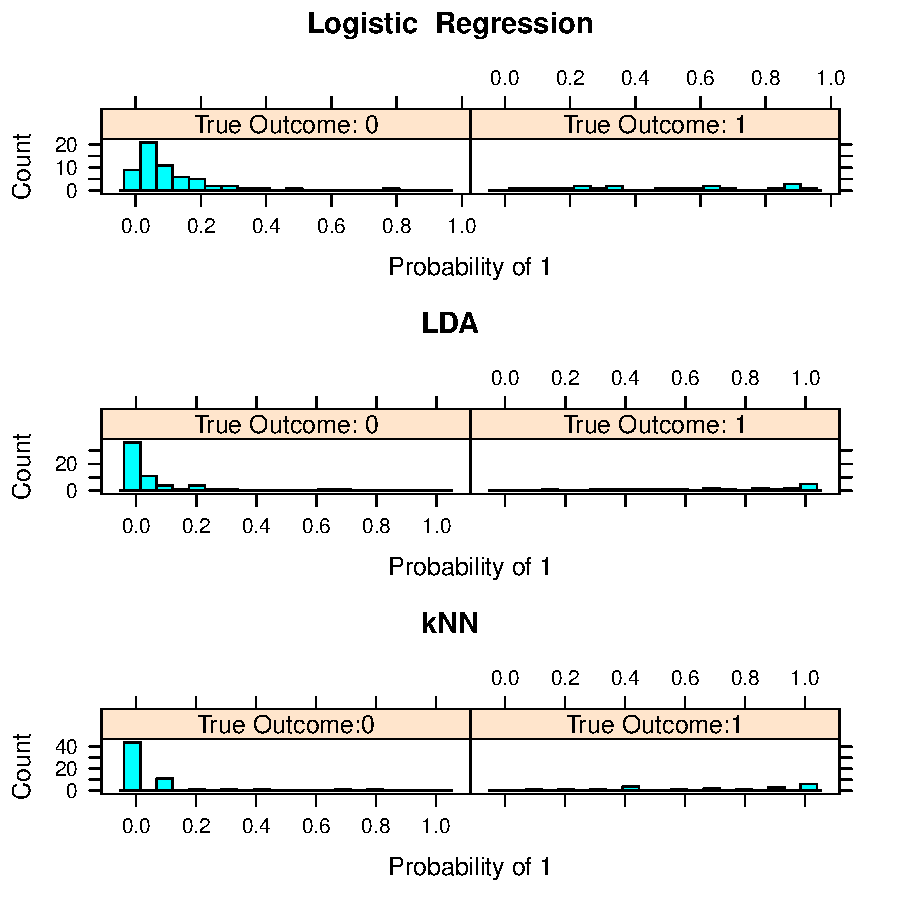
\includegraphics{week5-010}

   \end{solution}
   
   \item  For kNN, identify optimal $k$ value by minimising classification error on test set. 
    \begin{solution}
\begin{Schunk}
\begin{Sinput}
> library(pROC)
> ROCFull <- roc(KNNresultsFull$obs, KNNresultsFull$prob)
> auc(ROCFull)
\end{Sinput}
\begin{Soutput}
Area under the curve: 0.9717
\end{Soutput}
\begin{Sinput}
> ci.auc(ROCFull)
\end{Sinput}
\begin{Soutput}
95% CI: 0.9417-1 (DeLong)
\end{Soutput}
\begin{Sinput}
> plot(ROCFull, legacy.axes = TRUE, col ="black")
\end{Sinput}
\end{Schunk}
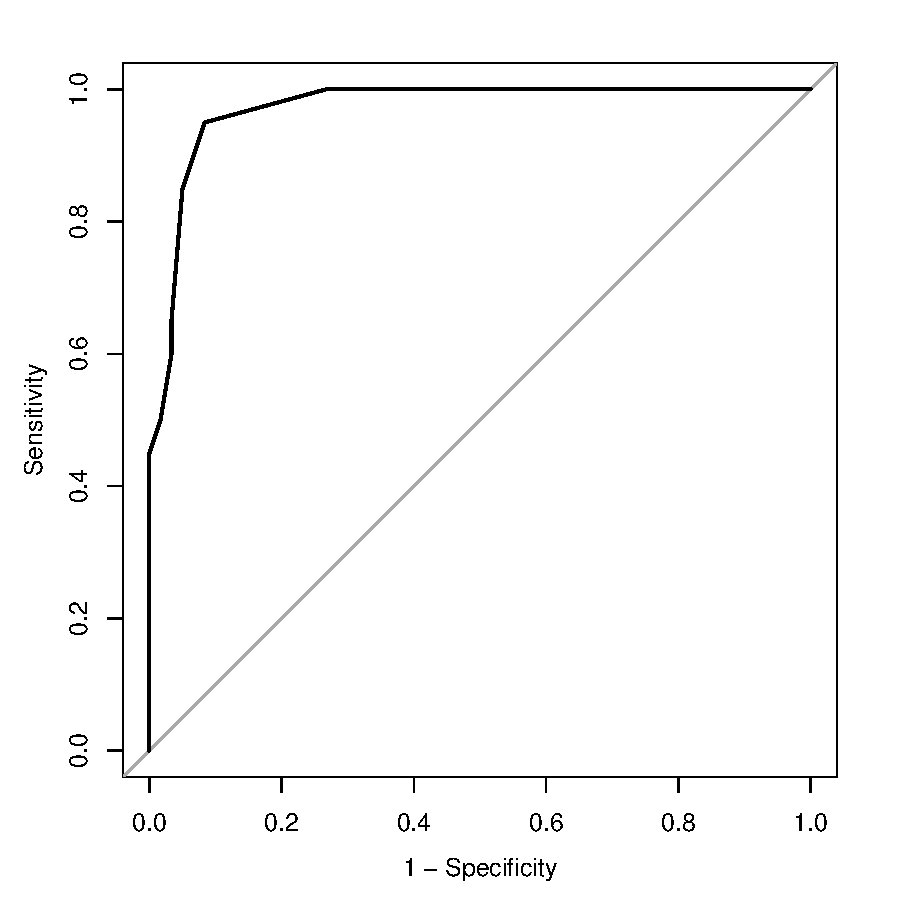
\includegraphics{week5-011}
As we can see from the Sensitivy Specificity Curve $k=9$ is the optimal based on minimising classification errors.   
    \end{solution}
   \item Now we used test set to select optimal k, is it still valid to use this test set to evaluate
the performance of our optimised kNN classifier? Why or why not?
\begin{solution}
No, it is best to use a different test set drawn again from the sample, albeit ensuring that it is a balanced data set.
\end{solution}
    \end{enumerate}

\end{document}
